\documentclass[twoside]{book}

% Packages required by doxygen
\usepackage{fixltx2e}
\usepackage{calc}
\usepackage{doxygen}
\usepackage{graphicx}
\usepackage[utf8]{inputenc}
\usepackage{makeidx}
\usepackage{multicol}
\usepackage{multirow}
\PassOptionsToPackage{warn}{textcomp}
\usepackage{textcomp}
\usepackage[nointegrals]{wasysym}
\usepackage[table]{xcolor}

% NLS support packages
\usepackage[french]{babel}

% Font selection
\usepackage[T1]{fontenc}
\usepackage{mathptmx}
\usepackage[scaled=.90]{helvet}
\usepackage{courier}
\usepackage{amssymb}
\usepackage{sectsty}
\renewcommand{\familydefault}{\sfdefault}
\allsectionsfont{%
  \fontseries{bc}\selectfont%
  \color{darkgray}%
}
\renewcommand{\DoxyLabelFont}{%
  \fontseries{bc}\selectfont%
  \color{darkgray}%
}
\newcommand{\+}{\discretionary{\mbox{\scriptsize$\hookleftarrow$}}{}{}}

% Page & text layout
\usepackage{geometry}
\geometry{%
  a4paper,%
  top=2.5cm,%
  bottom=2.5cm,%
  left=2.5cm,%
  right=2.5cm%
}
\tolerance=750
\hfuzz=15pt
\hbadness=750
\setlength{\emergencystretch}{15pt}
\setlength{\parindent}{0cm}
\setlength{\parskip}{0.2cm}
\makeatletter
\renewcommand{\paragraph}{%
  \@startsection{paragraph}{4}{0ex}{-1.0ex}{1.0ex}{%
    \normalfont\normalsize\bfseries\SS@parafont%
  }%
}
\renewcommand{\subparagraph}{%
  \@startsection{subparagraph}{5}{0ex}{-1.0ex}{1.0ex}{%
    \normalfont\normalsize\bfseries\SS@subparafont%
  }%
}
\makeatother

% Headers & footers
\usepackage{fancyhdr}
\pagestyle{fancyplain}
\fancyhead[LE]{\fancyplain{}{\bfseries\thepage}}
\fancyhead[CE]{\fancyplain{}{}}
\fancyhead[RE]{\fancyplain{}{\bfseries\leftmark}}
\fancyhead[LO]{\fancyplain{}{\bfseries\rightmark}}
\fancyhead[CO]{\fancyplain{}{}}
\fancyhead[RO]{\fancyplain{}{\bfseries\thepage}}
\fancyfoot[LE]{\fancyplain{}{}}
\fancyfoot[CE]{\fancyplain{}{}}
\fancyfoot[RE]{\fancyplain{}{\bfseries\scriptsize Généré le Jeudi 12 Octobre 2017 11\+:52\+:44 pour appli\+Note par Doxygen }}
\fancyfoot[LO]{\fancyplain{}{\bfseries\scriptsize Généré le Jeudi 12 Octobre 2017 11\+:52\+:44 pour appli\+Note par Doxygen }}
\fancyfoot[CO]{\fancyplain{}{}}
\fancyfoot[RO]{\fancyplain{}{}}
\renewcommand{\footrulewidth}{0.4pt}
\renewcommand{\chaptermark}[1]{%
  \markboth{#1}{}%
}
\renewcommand{\sectionmark}[1]{%
  \markright{\thesection\ #1}%
}

% Indices & bibliography
\usepackage{natbib}
\usepackage[titles]{tocloft}
\setcounter{tocdepth}{3}
\setcounter{secnumdepth}{5}
\makeindex

% Hyperlinks (required, but should be loaded last)
\usepackage{ifpdf}
\ifpdf
  \usepackage[pdftex,pagebackref=true]{hyperref}
\else
  \usepackage[ps2pdf,pagebackref=true]{hyperref}
\fi
\hypersetup{%
  colorlinks=true,%
  linkcolor=blue,%
  citecolor=blue,%
  unicode%
}

% Custom commands
\newcommand{\clearemptydoublepage}{%
  \newpage{\pagestyle{empty}\cleardoublepage}%
}


%===== C O N T E N T S =====

\begin{document}

% Titlepage & ToC
\hypersetup{pageanchor=false,
             bookmarks=true,
             bookmarksnumbered=true,
             pdfencoding=unicode
            }
\pagenumbering{roman}
\begin{titlepage}
\vspace*{7cm}
\begin{center}%
{\Large appli\+Note \\[1ex]\large 0.\+1 }\\
\vspace*{1cm}
{\large Généré par Doxygen 1.8.8}\\
\vspace*{0.5cm}
{\small Jeudi 12 Octobre 2017 11:52:44}\\
\end{center}
\end{titlepage}
\clearemptydoublepage
\tableofcontents
\clearemptydoublepage
\pagenumbering{arabic}
\hypersetup{pageanchor=true}

%--- Begin generated contents ---
\chapter{Index des classes}
\section{Liste des classes}
Liste des classes, structures, unions et interfaces avec une brève description \+:\begin{DoxyCompactList}
\item\contentsline{section}{\hyperlink{class_application}{Application} \\*Classe instanciée une fois dans le main }{\pageref{class_application}}{}
\item\contentsline{section}{\hyperlink{class_bulletin}{Bulletin} }{\pageref{class_bulletin}}{}
\item\contentsline{section}{\hyperlink{class_etudiant}{Etudiant} \\*Classe dont il peux exister plusieur instance dans la section }{\pageref{class_etudiant}}{}
\item\contentsline{section}{\hyperlink{class_evaluation}{Evaluation} }{\pageref{class_evaluation}}{}
\item\contentsline{section}{\hyperlink{class_matiere}{Matiere} \\*Classe dont il peux exister plusieur instance dans l'application }{\pageref{class_matiere}}{}
\item\contentsline{section}{\hyperlink{class_note}{Note} }{\pageref{class_note}}{}
\item\contentsline{section}{\hyperlink{class_section}{Section} \\*Classe dont il peux exister plusieur instance dans l'application }{\pageref{class_section}}{}
\end{DoxyCompactList}

\chapter{Index des fichiers}
\section{Liste des fichiers}
Liste de tous les fichiers documentés avec une brève description \+:\begin{DoxyCompactList}
\item\contentsline{section}{\hyperlink{application_8h}{application.\+h} }{\pageref{application_8h}}{}
\item\contentsline{section}{{\bfseries bulletin.\+h} }{\pageref{bulletin_8h}}{}
\item\contentsline{section}{\hyperlink{etudiant_8h}{etudiant.\+h} }{\pageref{etudiant_8h}}{}
\item\contentsline{section}{{\bfseries evaluation.\+h} }{\pageref{evaluation_8h}}{}
\item\contentsline{section}{\hyperlink{matiere_8h}{matiere.\+h} }{\pageref{matiere_8h}}{}
\item\contentsline{section}{{\bfseries note.\+h} }{\pageref{note_8h}}{}
\item\contentsline{section}{\hyperlink{section_8h}{section.\+h} }{\pageref{section_8h}}{}
\end{DoxyCompactList}

\chapter{Documentation des classes}
\hypertarget{class_application}{\section{Référence de la classe Application}
\label{class_application}\index{Application@{Application}}
}


classe instanciée une fois dans le main  




{\ttfamily \#include $<$application.\+h$>$}

\subsection*{Fonctions membres publiques}
\begin{DoxyCompactItemize}
\item 
\hypertarget{class_application_abc0b42851a0a44aa9d9150604c84bcc2}{void \hyperlink{class_application_abc0b42851a0a44aa9d9150604c84bcc2}{afficher\+Matiere} ()}\label{class_application_abc0b42851a0a44aa9d9150604c84bcc2}

\begin{DoxyCompactList}\small\item\em action qui permet d'afficher toutes les matières à l'utilisateur \end{DoxyCompactList}\item 
\hypertarget{class_application_a68965449404743bf1add056784d6cf81}{void \hyperlink{class_application_a68965449404743bf1add056784d6cf81}{run} ()}\label{class_application_a68965449404743bf1add056784d6cf81}

\begin{DoxyCompactList}\small\item\em méthode présent dans le main qui permet au menu principal de l'application de tourner \end{DoxyCompactList}\item 
\hypertarget{class_application_a0e74957eda5f689046bf6674a9795468}{vector$<$ \hyperlink{class_matiere}{Matiere} $\ast$ $>$ \hyperlink{class_application_a0e74957eda5f689046bf6674a9795468}{get\+Les\+Matieres} ()}\label{class_application_a0e74957eda5f689046bf6674a9795468}

\begin{DoxyCompactList}\small\item\em méthode qui permet de récupérer toutes les matières ajouter par l'utilisateur dans le menu secondaire de la section \end{DoxyCompactList}\end{DoxyCompactItemize}
\subsection*{Fonctions membres privées}
\begin{DoxyCompactItemize}
\item 
\hypertarget{class_application_adfcba0e50f0c263cdde8017329baaf37}{void \hyperlink{class_application_adfcba0e50f0c263cdde8017329baaf37}{afficher\+Menu1} ()}\label{class_application_adfcba0e50f0c263cdde8017329baaf37}

\begin{DoxyCompactList}\small\item\em permet d'afficher le menu principal de l'application \end{DoxyCompactList}\item 
\hypertarget{class_application_a019c961894cce7c789070053083b4c3f}{char \hyperlink{class_application_a019c961894cce7c789070053083b4c3f}{saisie\+Choix} ()}\label{class_application_a019c961894cce7c789070053083b4c3f}

\begin{DoxyCompactList}\small\item\em permet à l'utilisateur de saisir son choix parmit les actions du menu principal \end{DoxyCompactList}\item 
\hypertarget{class_application_a0d957c3dd1a2d88b2c9d5c01bd123a9d}{void \hyperlink{class_application_a0d957c3dd1a2d88b2c9d5c01bd123a9d}{action\+Choix} (char le\+Choix)}\label{class_application_a0d957c3dd1a2d88b2c9d5c01bd123a9d}

\begin{DoxyCompactList}\small\item\em permet d'appelé la méthode du choix de l'action choisi par l'utilisateur \end{DoxyCompactList}\item 
\hypertarget{class_application_a08280a27faf4c8dcae825cc2bf87845d}{void \hyperlink{class_application_a08280a27faf4c8dcae825cc2bf87845d}{ajouter\+Section} ()}\label{class_application_a08280a27faf4c8dcae825cc2bf87845d}

\begin{DoxyCompactList}\small\item\em action qui permet à l'utilisateur d'ajouter une section \end{DoxyCompactList}\item 
\hypertarget{class_application_a0096f4706fc9c1ede19b3c7a91673898}{void \hyperlink{class_application_a0096f4706fc9c1ede19b3c7a91673898}{afficher\+Section} ()}\label{class_application_a0096f4706fc9c1ede19b3c7a91673898}

\begin{DoxyCompactList}\small\item\em action qui permet d'afficher toutes les sections à l'utilisateur \end{DoxyCompactList}\item 
\hypertarget{class_application_aa8394d87b6d8aeedf585e057ab3b4440}{\hyperlink{class_section}{Section} $\ast$ \hyperlink{class_application_aa8394d87b6d8aeedf585e057ab3b4440}{select\+Section} ()}\label{class_application_aa8394d87b6d8aeedf585e057ab3b4440}

\begin{DoxyCompactList}\small\item\em action qui permet de selectionner la section choisi afin d'acceder au menu secondaire de la section \end{DoxyCompactList}\item 
\hypertarget{class_application_aab7ab676955bd4dc68f1a2fbb59d405a}{void \hyperlink{class_application_aab7ab676955bd4dc68f1a2fbb59d405a}{ajouter\+Matiere} ()}\label{class_application_aab7ab676955bd4dc68f1a2fbb59d405a}

\begin{DoxyCompactList}\small\item\em action qui permet à l'utilisateur d'ajouter une matière \end{DoxyCompactList}\item 
\hypertarget{class_application_a49e81e1531a1a19ff6f422ea6bfd474b}{void \hyperlink{class_application_a49e81e1531a1a19ff6f422ea6bfd474b}{quitter} ()}\label{class_application_a49e81e1531a1a19ff6f422ea6bfd474b}

\begin{DoxyCompactList}\small\item\em action qui permet à l'utilisateur de quitter l'application \end{DoxyCompactList}\end{DoxyCompactItemize}
\subsection*{Attributs privés}
\begin{DoxyCompactItemize}
\item 
\hypertarget{class_application_a689a25902c2e34e61bdd122d4c92d941}{vector$<$ \hyperlink{class_section}{Section} $>$ \hyperlink{class_application_a689a25902c2e34e61bdd122d4c92d941}{vect\+Section}}\label{class_application_a689a25902c2e34e61bdd122d4c92d941}

\begin{DoxyCompactList}\small\item\em vide au départ, il contient l'ensemble des sections ajouté par l'utilisateur \end{DoxyCompactList}\item 
\hypertarget{class_application_ac5a9a7ed9aab9411814d9cd53af9175d}{vector$<$ \hyperlink{class_matiere}{Matiere} $>$ \hyperlink{class_application_ac5a9a7ed9aab9411814d9cd53af9175d}{vect\+Matiere}}\label{class_application_ac5a9a7ed9aab9411814d9cd53af9175d}

\begin{DoxyCompactList}\small\item\em vide au départ, il contient l'ensemble de toutes les matières ajouté par l'utilisateur \end{DoxyCompactList}\end{DoxyCompactItemize}


\subsection{Description détaillée}
classe instanciée une fois dans le main 

une section est une class d'élèves avec ses propres matières et ses propres élèves / une matière est un cours au quels les élèves participent selon leur section 

La documentation de cette classe a été générée à partir des fichiers suivants \+:\begin{DoxyCompactItemize}
\item 
\hyperlink{application_8h}{application.\+h}\item 
application.\+cpp\end{DoxyCompactItemize}

\hypertarget{class_bulletin}{\section{Référence de la classe Bulletin}
\label{class_bulletin}\index{Bulletin@{Bulletin}}
}
\subsection*{Fonctions membres publiques}
\begin{DoxyCompactItemize}
\item 
\hypertarget{class_bulletin_a205129b160a08aa026ac8d5f9b5fd4c8}{string {\bfseries get\+Appreciation} ()}\label{class_bulletin_a205129b160a08aa026ac8d5f9b5fd4c8}

\item 
\hypertarget{class_bulletin_a8c80b89f22792e5706e6276f882daf44}{void {\bfseries set\+Appreciation} (int this\+Appreciation)}\label{class_bulletin_a8c80b89f22792e5706e6276f882daf44}

\item 
\hypertarget{class_bulletin_a9c98ddfef1e472439bccf90a68431527}{void {\bfseries display} ()}\label{class_bulletin_a9c98ddfef1e472439bccf90a68431527}

\item 
\hypertarget{class_bulletin_aa417e7a45dd7f6d216e97d516345feaf}{void {\bfseries input} ()}\label{class_bulletin_aa417e7a45dd7f6d216e97d516345feaf}

\end{DoxyCompactItemize}
\subsection*{Attributs privés}
\begin{DoxyCompactItemize}
\item 
\hypertarget{class_bulletin_a41e708509d0a07b16fada453da8cc01f}{vector$<$ string $>$ {\bfseries vect\+Apreciation}}\label{class_bulletin_a41e708509d0a07b16fada453da8cc01f}

\end{DoxyCompactItemize}


La documentation de cette classe a été générée à partir du fichier suivant \+:\begin{DoxyCompactItemize}
\item 
bulletin.\+h\end{DoxyCompactItemize}

\hypertarget{class_etudiant}{\section{Référence de la classe Etudiant}
\label{class_etudiant}\index{Etudiant@{Etudiant}}
}


classe dont il peux exister plusieur instance dans la section  




{\ttfamily \#include $<$etudiant.\+h$>$}

\subsection*{Fonctions membres publiques}
\begin{DoxyCompactItemize}
\item 
\hypertarget{class_etudiant_afdc3229a90d775ed4af4fb40fa647522}{string \hyperlink{class_etudiant_afdc3229a90d775ed4af4fb40fa647522}{get\+Nom} ()}\label{class_etudiant_afdc3229a90d775ed4af4fb40fa647522}

\begin{DoxyCompactList}\small\item\em methode de getteur qui permet d'aller rechercher la valeur saisie par l'utilisateur lors de la saisi du nom de l'étudiant \end{DoxyCompactList}\item 
\hypertarget{class_etudiant_a626fa65bbdbc09a5e7e5864781545aa4}{string \hyperlink{class_etudiant_a626fa65bbdbc09a5e7e5864781545aa4}{get\+Prenom} ()}\label{class_etudiant_a626fa65bbdbc09a5e7e5864781545aa4}

\begin{DoxyCompactList}\small\item\em methode de getteur qui permet d'aller rechercher la valeur saisie par l'utilisateur lors de la saisi du prénom de l'étudiant \end{DoxyCompactList}\item 
\hypertarget{class_etudiant_adac75b58619d7f0991a0cccb6557e194}{string \hyperlink{class_etudiant_adac75b58619d7f0991a0cccb6557e194}{get\+Date\+Naissance} ()}\label{class_etudiant_adac75b58619d7f0991a0cccb6557e194}

\begin{DoxyCompactList}\small\item\em methode de getteur qui permet d'aller rechercher la valeur saisie par l'utilisateur lors de la saisi de la date de naissance de l'étudiant \end{DoxyCompactList}\item 
\hypertarget{class_etudiant_a3f588d55135f5d794ae47f23c1b7a9c7}{int \hyperlink{class_etudiant_a3f588d55135f5d794ae47f23c1b7a9c7}{get\+Nb\+Absence} ()}\label{class_etudiant_a3f588d55135f5d794ae47f23c1b7a9c7}

\begin{DoxyCompactList}\small\item\em methode de getteur qui permet d'aller rechercher la valeur saisie par l'utilisateur lors de la saisi d'un évaluation que l'étudiant a loupé \end{DoxyCompactList}\item 
\hypertarget{class_etudiant_a86e74508e1780e6521121ed1afbf3987}{void \hyperlink{class_etudiant_a86e74508e1780e6521121ed1afbf3987}{set\+Nom} (string this\+Nom)}\label{class_etudiant_a86e74508e1780e6521121ed1afbf3987}

\begin{DoxyCompactList}\small\item\em methode de setteur qui permet de modifier la valeur saisie par l'utilisateur pour le nom de l'étudiant \end{DoxyCompactList}\item 
\hypertarget{class_etudiant_a02fef0e3259e82cada9293331454eba9}{void \hyperlink{class_etudiant_a02fef0e3259e82cada9293331454eba9}{set\+Prenom} (string this\+Prenom)}\label{class_etudiant_a02fef0e3259e82cada9293331454eba9}

\begin{DoxyCompactList}\small\item\em methode de setteur qui permet de modifier la valeur saisie par l'utilisateur pour le prénom de l'étudiant \end{DoxyCompactList}\item 
\hypertarget{class_etudiant_a3cd8cbebc9426c70289953a474dfa5ee}{void \hyperlink{class_etudiant_a3cd8cbebc9426c70289953a474dfa5ee}{set\+Old} (string this\+Date\+Naissance)}\label{class_etudiant_a3cd8cbebc9426c70289953a474dfa5ee}

\begin{DoxyCompactList}\small\item\em methode de setteur qui permet de modifier la valeur saisie par l'utilisateur pour la date de naissance de l'étudiant \end{DoxyCompactList}\item 
\hypertarget{class_etudiant_a36f5dcdac557fa14dfa5a3808552cc53}{void \hyperlink{class_etudiant_a36f5dcdac557fa14dfa5a3808552cc53}{set\+Nb\+Absence} (int this\+Nb\+Absebce)}\label{class_etudiant_a36f5dcdac557fa14dfa5a3808552cc53}

\begin{DoxyCompactList}\small\item\em methode de setteur qui permet de modifier la valeur des absences de l'étudiant \end{DoxyCompactList}\item 
\hypertarget{class_etudiant_afb95ac0c74157e6065e1de603c54381c}{void \hyperlink{class_etudiant_afb95ac0c74157e6065e1de603c54381c}{display} ()}\label{class_etudiant_afb95ac0c74157e6065e1de603c54381c}

\begin{DoxyCompactList}\small\item\em methode d'affichage d'un étudiant appelé dans le menu secondaire \end{DoxyCompactList}\item 
\hypertarget{class_etudiant_a37433540e5c7b724de0964a5ecbbead8}{void \hyperlink{class_etudiant_a37433540e5c7b724de0964a5ecbbead8}{input} ()}\label{class_etudiant_a37433540e5c7b724de0964a5ecbbead8}

\begin{DoxyCompactList}\small\item\em methode de saisie d'un étudiant appelé dans le menu secondaire \end{DoxyCompactList}\end{DoxyCompactItemize}
\subsection*{Attributs privés}
\begin{DoxyCompactItemize}
\item 
\hypertarget{class_etudiant_a51185c35f25f27013812b897695e50cf}{string \hyperlink{class_etudiant_a51185c35f25f27013812b897695e50cf}{nom}}\label{class_etudiant_a51185c35f25f27013812b897695e50cf}

\begin{DoxyCompactList}\small\item\em contient ce qu'a entré l'utilisateur lors de l'ajout d'un étudiant et conrrespond au nom de famille de l'étudiant \end{DoxyCompactList}\item 
\hypertarget{class_etudiant_a014830eb28c8d8be56701df7141120b6}{string \hyperlink{class_etudiant_a014830eb28c8d8be56701df7141120b6}{prenom}}\label{class_etudiant_a014830eb28c8d8be56701df7141120b6}

\begin{DoxyCompactList}\small\item\em contient ce qu'a entré l'utilisateur lors de l'ajout d'un étudiant et conrrespond au prénom de l'étudiant \end{DoxyCompactList}\item 
\hypertarget{class_etudiant_ae0252be67ef5b4fcaf0180699913751b}{string \hyperlink{class_etudiant_ae0252be67ef5b4fcaf0180699913751b}{date\+Naissance}}\label{class_etudiant_ae0252be67ef5b4fcaf0180699913751b}

\begin{DoxyCompactList}\small\item\em contient ce qu'a entré l'utilisateur lors de l'ajout d'un étudiant et conrrespond a la date de naissance (J\+J/\+M\+M/\+A\+A\+A) de l'étudiant \end{DoxyCompactList}\item 
\hypertarget{class_etudiant_a16ed7b766d6a5f0e6cf476cc033ffe6e}{int \hyperlink{class_etudiant_a16ed7b766d6a5f0e6cf476cc033ffe6e}{nb\+Absence}}\label{class_etudiant_a16ed7b766d6a5f0e6cf476cc033ffe6e}

\begin{DoxyCompactList}\small\item\em contient le nombre d'absence de l'étudiant selon les évaluation loupé, saisie par l'utilisateurs lors d'un ajout d'une évaluation \end{DoxyCompactList}\item 
\hypertarget{class_etudiant_a11eda3a9ed55f23aab1357ac0d47ed26}{vector$<$ \hyperlink{class_bulletin}{Bulletin} $>$ \hyperlink{class_etudiant_a11eda3a9ed55f23aab1357ac0d47ed26}{vect\+Bulletin}}\label{class_etudiant_a11eda3a9ed55f23aab1357ac0d47ed26}

\begin{DoxyCompactList}\small\item\em vide au départ, il contient les deux bulletin de l'étudiant de l'année (1 par semestre), qui varie selon l'étudiant \end{DoxyCompactList}\end{DoxyCompactItemize}


\subsection{Description détaillée}
classe dont il peux exister plusieur instance dans la section 

un élève est une personne, un élève qui fait partie d'une section et participe à plusieurs matières / nb\+Absance est le nombre d'absence d'un élève selon les evaluation qu'il à loupé 

La documentation de cette classe a été générée à partir des fichiers suivants \+:\begin{DoxyCompactItemize}
\item 
\hyperlink{etudiant_8h}{etudiant.\+h}\item 
etudiant.\+cpp\end{DoxyCompactItemize}

\hypertarget{class_evaluation}{\section{Référence de la classe Evaluation}
\label{class_evaluation}\index{Evaluation@{Evaluation}}
}


Graphe de collaboration de Evaluation\+:\nopagebreak
\begin{figure}[H]
\begin{center}
\leavevmode
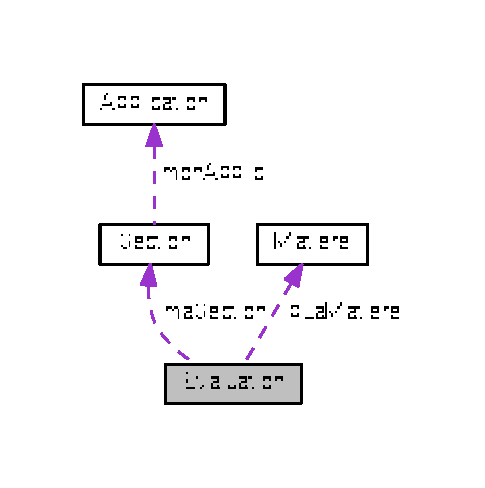
\includegraphics[width=233pt]{class_evaluation__coll__graph}
\end{center}
\end{figure}
\subsection*{Fonctions membres publiques}
\begin{DoxyCompactItemize}
\item 
\hypertarget{class_evaluation_a6fbb1585de7c53a1d5a3cff19c1b20c9}{string {\bfseries get\+Ref\+Eval} ()}\label{class_evaluation_a6fbb1585de7c53a1d5a3cff19c1b20c9}

\item 
\hypertarget{class_evaluation_a663623cd21f48ea4815adbe4ff868531}{int {\bfseries get\+Semestre\+Eval} ()}\label{class_evaluation_a663623cd21f48ea4815adbe4ff868531}

\item 
\hypertarget{class_evaluation_ac5a47801531e58bc2621663e7452f1c2}{void {\bfseries set\+Ref\+Eval} (string this\+Eval)}\label{class_evaluation_ac5a47801531e58bc2621663e7452f1c2}

\item 
\hypertarget{class_evaluation_ad22320bf30d0ce0a276c0f1a7cc917e4}{void {\bfseries set\+Semestre\+Eval} (int this\+Semestre)}\label{class_evaluation_ad22320bf30d0ce0a276c0f1a7cc917e4}

\item 
\hypertarget{class_evaluation_a2dfd725e201bf995fac36111ad12d6ac}{void {\bfseries display} ()}\label{class_evaluation_a2dfd725e201bf995fac36111ad12d6ac}

\item 
\hypertarget{class_evaluation_a3599a3e29cf65a30a2deef8d4a0731ca}{void {\bfseries input} ()}\label{class_evaluation_a3599a3e29cf65a30a2deef8d4a0731ca}

\item 
\hypertarget{class_evaluation_a05813c0c8638a54bf524e84566cf3676}{\hyperlink{class_section}{Section} $\ast$ {\bfseries get\+P\+Section} ()}\label{class_evaluation_a05813c0c8638a54bf524e84566cf3676}

\item 
\hypertarget{class_evaluation_a7338edac80f158f18481f965710706bc}{{\bfseries Evaluation} (\hyperlink{class_section}{Section} $\ast$)}\label{class_evaluation_a7338edac80f158f18481f965710706bc}

\end{DoxyCompactItemize}
\subsection*{Attributs privés}
\begin{DoxyCompactItemize}
\item 
\hypertarget{class_evaluation_aba14a650a0ee11f25805adae67627002}{string {\bfseries ref\+Eval}}\label{class_evaluation_aba14a650a0ee11f25805adae67627002}

\item 
\hypertarget{class_evaluation_afb9abd8c900951793e3a9c822a07ea62}{int {\bfseries semestre\+Eval}}\label{class_evaluation_afb9abd8c900951793e3a9c822a07ea62}

\item 
\hypertarget{class_evaluation_ad5f4d301c80076389e2ea31dfd7f09b1}{\hyperlink{class_matiere}{Matiere} $\ast$ {\bfseries p\+La\+Matiere}}\label{class_evaluation_ad5f4d301c80076389e2ea31dfd7f09b1}

\item 
\hypertarget{class_evaluation_ad26840cec05aea45af3b1164c55a7557}{vector$<$ \hyperlink{class_note}{Note} $>$ {\bfseries vect\+Note}}\label{class_evaluation_ad26840cec05aea45af3b1164c55a7557}

\item 
\hypertarget{class_evaluation_afff6a111c7954292f1b36aaa2298bac6}{\hyperlink{class_section}{Section} $\ast$ {\bfseries ma\+Section}}\label{class_evaluation_afff6a111c7954292f1b36aaa2298bac6}

\end{DoxyCompactItemize}


La documentation de cette classe a été générée à partir des fichiers suivants \+:\begin{DoxyCompactItemize}
\item 
evaluation.\+h\item 
evaluation.\+cpp\end{DoxyCompactItemize}

\hypertarget{class_matiere}{\section{Référence de la classe Matiere}
\label{class_matiere}\index{Matiere@{Matiere}}
}


classe dont il peux exister plusieur instance dans l'application  




{\ttfamily \#include $<$matiere.\+h$>$}

\subsection*{Fonctions membres publiques}
\begin{DoxyCompactItemize}
\item 
\hypertarget{class_matiere_a70412c2670239d7b6db78e5f631e04b2}{string \hyperlink{class_matiere_a70412c2670239d7b6db78e5f631e04b2}{get\+Libelle\+Matiere} ()}\label{class_matiere_a70412c2670239d7b6db78e5f631e04b2}

\begin{DoxyCompactList}\small\item\em methode de getteur qui permet d'aller rechercher la valeur saisie par l'utilisateur lors de la saisi du libelle de la matière \end{DoxyCompactList}\item 
\hypertarget{class_matiere_a0cfae521cb6b0a4de029e8f5c493c163}{void \hyperlink{class_matiere_a0cfae521cb6b0a4de029e8f5c493c163}{set\+Libelle\+Matiere} (string this\+Matiere)}\label{class_matiere_a0cfae521cb6b0a4de029e8f5c493c163}

\begin{DoxyCompactList}\small\item\em methode de setteur qui permet de modifier la valeur saisie par l'utilisateur pour le libelle de la matière \end{DoxyCompactList}\item 
\hypertarget{class_matiere_a83c7ad70642d1c15c2b43c5e6c2823d2}{void \hyperlink{class_matiere_a83c7ad70642d1c15c2b43c5e6c2823d2}{display} ()}\label{class_matiere_a83c7ad70642d1c15c2b43c5e6c2823d2}

\begin{DoxyCompactList}\small\item\em methode d'affichage d'une matière appelé dans le menu principal \end{DoxyCompactList}\item 
\hypertarget{class_matiere_a314ae9fc824027e032c9c02faf3ccc8f}{void \hyperlink{class_matiere_a314ae9fc824027e032c9c02faf3ccc8f}{input} ()}\label{class_matiere_a314ae9fc824027e032c9c02faf3ccc8f}

\begin{DoxyCompactList}\small\item\em methode de saisie d'une section appelé dans le menu principal \end{DoxyCompactList}\end{DoxyCompactItemize}
\subsection*{Attributs privés}
\begin{DoxyCompactItemize}
\item 
\hypertarget{class_matiere_a480270db0295385a1bee7c97918c47c9}{string \hyperlink{class_matiere_a480270db0295385a1bee7c97918c47c9}{libelle\+Matiere}}\label{class_matiere_a480270db0295385a1bee7c97918c47c9}

\begin{DoxyCompactList}\small\item\em contient ce qu'a entré l'utilisateur lors de l'ajout d'une matière et conrrespond au libelle de la matière \end{DoxyCompactList}\end{DoxyCompactItemize}


\subsection{Description détaillée}
classe dont il peux exister plusieur instance dans l'application 

une matière est un cours au quels les élèves participent selon leur section (ex\+: Mathématique) 

La documentation de cette classe a été générée à partir des fichiers suivants \+:\begin{DoxyCompactItemize}
\item 
\hyperlink{matiere_8h}{matiere.\+h}\item 
matiere.\+cpp\end{DoxyCompactItemize}

\hypertarget{class_note}{\section{Référence de la classe Note}
\label{class_note}\index{Note@{Note}}
}


Graphe de collaboration de Note\+:
\nopagebreak
\begin{figure}[H]
\begin{center}
\leavevmode
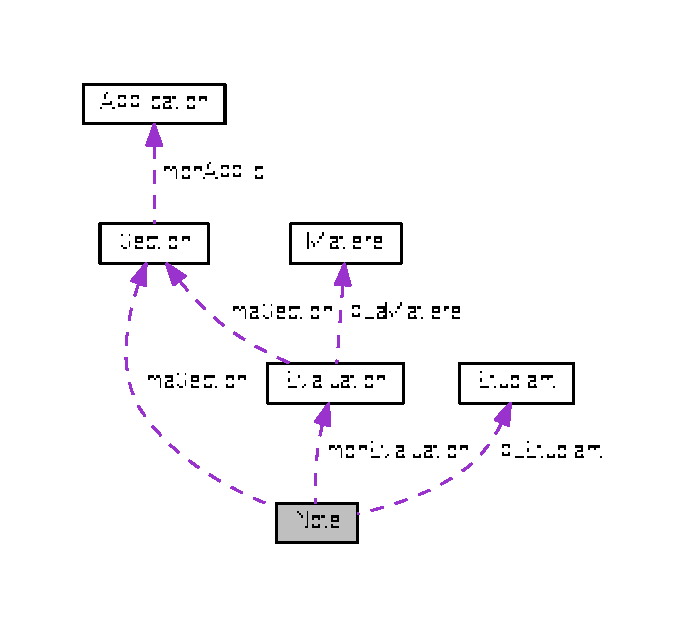
\includegraphics[width=330pt]{class_note__coll__graph}
\end{center}
\end{figure}
\subsection*{Fonctions membres publiques}
\begin{DoxyCompactItemize}
\item 
\hypertarget{class_note_a880f020b1e9fe974fd2a3064af3257c6}{int {\bfseries get\+Note} ()}\label{class_note_a880f020b1e9fe974fd2a3064af3257c6}

\item 
\hypertarget{class_note_a2624f81d3da32203d65804d4c0d7379e}{void {\bfseries set\+Note} (int this\+Note)}\label{class_note_a2624f81d3da32203d65804d4c0d7379e}

\item 
\hypertarget{class_note_aa2e4741a587cc0f44127e722e3dd6d6f}{void {\bfseries display} ()}\label{class_note_aa2e4741a587cc0f44127e722e3dd6d6f}

\item 
\hypertarget{class_note_a60e3344a645763b9bac160249e202206}{void {\bfseries input} ()}\label{class_note_a60e3344a645763b9bac160249e202206}

\item 
\hypertarget{class_note_a9e1747b439abeb626890a646f7c17a8d}{{\bfseries Note} (\hyperlink{class_evaluation}{Evaluation} $\ast$)}\label{class_note_a9e1747b439abeb626890a646f7c17a8d}

\end{DoxyCompactItemize}
\subsection*{Attributs privés}
\begin{DoxyCompactItemize}
\item 
\hypertarget{class_note_a3cb5f22dd5374f4e3c59c5f11dc7fbfb}{int {\bfseries note}}\label{class_note_a3cb5f22dd5374f4e3c59c5f11dc7fbfb}

\item 
\hypertarget{class_note_af0bd8055a09d8548b29611ab579419be}{\hyperlink{class_etudiant}{Etudiant} $\ast$ {\bfseries p\+L\+Etudiant}}\label{class_note_af0bd8055a09d8548b29611ab579419be}

\item 
\hypertarget{class_note_a6e57712bda6065467eb09ea96898b428}{\hyperlink{class_section}{Section} $\ast$ {\bfseries ma\+Section}}\label{class_note_a6e57712bda6065467eb09ea96898b428}

\item 
\hypertarget{class_note_a37ac6f84cda46c4c25ea8483836dd2d4}{\hyperlink{class_evaluation}{Evaluation} $\ast$ {\bfseries mon\+Evaluation}}\label{class_note_a37ac6f84cda46c4c25ea8483836dd2d4}

\end{DoxyCompactItemize}


La documentation de cette classe a été générée à partir des fichiers suivants \+:\begin{DoxyCompactItemize}
\item 
note.\+h\item 
note.\+cpp\end{DoxyCompactItemize}

\hypertarget{class_section}{\section{Référence de la classe Section}
\label{class_section}\index{Section@{Section}}
}


classe dont il peux exister plusieur instance dans l'application  




{\ttfamily \#include $<$section.\+h$>$}



Graphe de collaboration de Section\+:\nopagebreak
\begin{figure}[H]
\begin{center}
\leavevmode
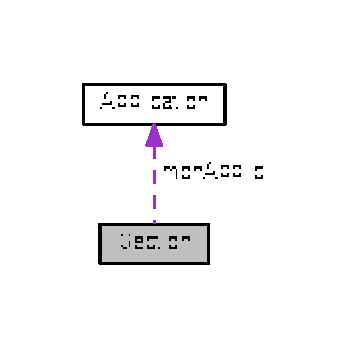
\includegraphics[width=166pt]{class_section__coll__graph}
\end{center}
\end{figure}
\subsection*{Fonctions membres publiques}
\begin{DoxyCompactItemize}
\item 
\hypertarget{class_section_ad60532fac7868faad0b9b6ae413c860d}{void \hyperlink{class_section_ad60532fac7868faad0b9b6ae413c860d}{run} ()}\label{class_section_ad60532fac7868faad0b9b6ae413c860d}

\begin{DoxyCompactList}\small\item\em méthode présent dans l'action du choix du menu princpal qui permet d'appeler et faire tourner le menu secondaire de l'application \end{DoxyCompactList}\item 
\hypertarget{class_section_ac23af2bd97ad21270f0a8a917ae9afa5}{void \hyperlink{class_section_ac23af2bd97ad21270f0a8a917ae9afa5}{afficher\+Menu2} ()}\label{class_section_ac23af2bd97ad21270f0a8a917ae9afa5}

\begin{DoxyCompactList}\small\item\em permet d'afficher le menu secondaire de l'application \end{DoxyCompactList}\item 
\hypertarget{class_section_a87e0a87007299f84d33af2e271996b73}{string \hyperlink{class_section_a87e0a87007299f84d33af2e271996b73}{get\+Libelle\+Section} ()}\label{class_section_a87e0a87007299f84d33af2e271996b73}

\begin{DoxyCompactList}\small\item\em methode de getteur qui permet d'aller rechercher la valeur saisie par l'utilisateur lors de la saisi du libelle de la section \end{DoxyCompactList}\item 
\hypertarget{class_section_a78293be5394560b79aeafed3bee45bcc}{int \hyperlink{class_section_a78293be5394560b79aeafed3bee45bcc}{get\+Coeff} ()}\label{class_section_a78293be5394560b79aeafed3bee45bcc}

\begin{DoxyCompactList}\small\item\em methode de getteur qui permet d'aller rechercher la valeur saisie par l'utilisateur lors de la saisi du coefficient de la matière \end{DoxyCompactList}\item 
\hypertarget{class_section_a60b70a27e31ab4418bb183c31b167092}{void \hyperlink{class_section_a60b70a27e31ab4418bb183c31b167092}{set\+Libelle\+Section} (string this\+Section)}\label{class_section_a60b70a27e31ab4418bb183c31b167092}

\begin{DoxyCompactList}\small\item\em methode de setteur qui permet de modifier la valeur saisie par l'utilisateur pour le libelle de la section \end{DoxyCompactList}\item 
\hypertarget{class_section_adb0132002130e3ba5270dfd8e566170b}{void \hyperlink{class_section_adb0132002130e3ba5270dfd8e566170b}{set\+Coeff} (int this\+Coeff)}\label{class_section_adb0132002130e3ba5270dfd8e566170b}

\begin{DoxyCompactList}\small\item\em methode de setteur qui permet de modifier la valeur saisie par l'utilisateur pour le ceofficient de la matière \end{DoxyCompactList}\item 
\hypertarget{class_section_a1f9ebccdb1937ca61a0d4adcde310832}{void \hyperlink{class_section_a1f9ebccdb1937ca61a0d4adcde310832}{display} ()}\label{class_section_a1f9ebccdb1937ca61a0d4adcde310832}

\begin{DoxyCompactList}\small\item\em methode d'affichage d'une section appelé dans le menu principal \end{DoxyCompactList}\item 
\hypertarget{class_section_a32e3a0a0682f01437a82ddbf7dd59b0a}{void \hyperlink{class_section_a32e3a0a0682f01437a82ddbf7dd59b0a}{input} ()}\label{class_section_a32e3a0a0682f01437a82ddbf7dd59b0a}

\begin{DoxyCompactList}\small\item\em methode de saisie d'une section appelé dans le menu principal \end{DoxyCompactList}\item 
\hypertarget{class_section_aa28c77d3c8f481f443df2841d43989f0}{vector$<$ \hyperlink{class_matiere}{Matiere} $\ast$ $>$ \hyperlink{class_section_aa28c77d3c8f481f443df2841d43989f0}{get\+Les\+Matieres\+De\+La\+Section} ()}\label{class_section_aa28c77d3c8f481f443df2841d43989f0}

\begin{DoxyCompactList}\small\item\em méthode qui permet de récupérer toutes les matières propre à cette section \end{DoxyCompactList}\item 
\hypertarget{class_section_ab6ec912b6d6dc3291d11f00527f08b7d}{vector$<$ \hyperlink{class_etudiant}{Etudiant} $\ast$ $>$ \hyperlink{class_section_ab6ec912b6d6dc3291d11f00527f08b7d}{get\+Les\+Etudiants\+De\+La\+Section} ()}\label{class_section_ab6ec912b6d6dc3291d11f00527f08b7d}

\begin{DoxyCompactList}\small\item\em méthode qui permet de récupérer tous les étudiants présent dans cette section \end{DoxyCompactList}\item 
\hypertarget{class_section_a1842f51fc609776feca3df6d45ce0ba1}{\hyperlink{class_section_a1842f51fc609776feca3df6d45ce0ba1}{Section} (\hyperlink{class_application}{Application} $\ast$)}\label{class_section_a1842f51fc609776feca3df6d45ce0ba1}

\begin{DoxyCompactList}\small\item\em constructeur qui permet de relier l'instance de cette section a l'application \end{DoxyCompactList}\end{DoxyCompactItemize}
\subsection*{Fonctions membres privées}
\begin{DoxyCompactItemize}
\item 
\hypertarget{class_section_a5f31422e8e43cf164de5ca56ba979f4a}{char \hyperlink{class_section_a5f31422e8e43cf164de5ca56ba979f4a}{saisie\+Choix} ()}\label{class_section_a5f31422e8e43cf164de5ca56ba979f4a}

\begin{DoxyCompactList}\small\item\em permet à l'utilisateur de saisir son choix parmit les actions du menu secondaire \end{DoxyCompactList}\item 
\hypertarget{class_section_aadf34655598195fa171b2c5a6f50a9c7}{void \hyperlink{class_section_aadf34655598195fa171b2c5a6f50a9c7}{action\+Choix} (char le\+Choix)}\label{class_section_aadf34655598195fa171b2c5a6f50a9c7}

\begin{DoxyCompactList}\small\item\em permet d'appelé la méthode du choix de l'action choisi par l'utilisateur \end{DoxyCompactList}\item 
\hypertarget{class_section_aca817449026803dfddfe01fb76b2a4d6}{void \hyperlink{class_section_aca817449026803dfddfe01fb76b2a4d6}{ajouter\+Etudiant} ()}\label{class_section_aca817449026803dfddfe01fb76b2a4d6}

\begin{DoxyCompactList}\small\item\em action qui permet à l'utilisateur d'ajouter un étudiant dans cette section \end{DoxyCompactList}\item 
\hypertarget{class_section_a762dcfde40a8821f21324d1ade96999b}{void \hyperlink{class_section_a762dcfde40a8821f21324d1ade96999b}{afficher\+Etudiant} ()}\label{class_section_a762dcfde40a8821f21324d1ade96999b}

\begin{DoxyCompactList}\small\item\em action qui permet d'afficher les élèves de cette section à l'utilisateur \end{DoxyCompactList}\item 
\hypertarget{class_section_af834dd53f188641f0b1cc24d7d18e919}{void \hyperlink{class_section_af834dd53f188641f0b1cc24d7d18e919}{ajouter\+Matiere} ()}\label{class_section_af834dd53f188641f0b1cc24d7d18e919}

\begin{DoxyCompactList}\small\item\em action qui permet à l'utilisateur d'affecter dans cette section une, matière existante dans l'application \end{DoxyCompactList}\item 
\hypertarget{class_section_a1debe78679287f470ce2ae2f8c5fd26d}{void \hyperlink{class_section_a1debe78679287f470ce2ae2f8c5fd26d}{afficher\+Matiere} ()}\label{class_section_a1debe78679287f470ce2ae2f8c5fd26d}

\begin{DoxyCompactList}\small\item\em action qui permet d'afficher les matières propre à cette section à l'utilisateur \end{DoxyCompactList}\item 
\hypertarget{class_section_a61635f5b31db8f7d3a779f751c117e56}{void \hyperlink{class_section_a61635f5b31db8f7d3a779f751c117e56}{ajouter\+Eval} ()}\label{class_section_a61635f5b31db8f7d3a779f751c117e56}

\begin{DoxyCompactList}\small\item\em action qui permet à l'utilisateur d'ajouter une évaluation dans cette section \end{DoxyCompactList}\item 
\hypertarget{class_section_a00d4f5165a2db3d1e30b7fa84c59027c}{void \hyperlink{class_section_a00d4f5165a2db3d1e30b7fa84c59027c}{afficher\+Eval} ()}\label{class_section_a00d4f5165a2db3d1e30b7fa84c59027c}

\begin{DoxyCompactList}\small\item\em action qui permet d'afficher les évaluations de cette section à l'utilisateur \end{DoxyCompactList}\item 
\hypertarget{class_section_a4bacd7ca9f2a152d966c0a19853887d3}{void \hyperlink{class_section_a4bacd7ca9f2a152d966c0a19853887d3}{retour} ()}\label{class_section_a4bacd7ca9f2a152d966c0a19853887d3}

\begin{DoxyCompactList}\small\item\em action qui permet à l'utilisateur de retourner au menu principal \end{DoxyCompactList}\end{DoxyCompactItemize}
\subsection*{Attributs privés}
\begin{DoxyCompactItemize}
\item 
\hypertarget{class_section_a8f6ad7b2f236367521e3578ed35ff3d5}{string \hyperlink{class_section_a8f6ad7b2f236367521e3578ed35ff3d5}{libelle\+Section}}\label{class_section_a8f6ad7b2f236367521e3578ed35ff3d5}

\begin{DoxyCompactList}\small\item\em contient ce qu'a entré l'utilisateur lors de l'ajout d'une section et conrrespond au libelle de la section \end{DoxyCompactList}\item 
\hypertarget{class_section_a387b69bedffb009e38d88cb272030bd4}{\hyperlink{class_application}{Application} $\ast$ \hyperlink{class_section_a387b69bedffb009e38d88cb272030bd4}{mon\+Applic}}\label{class_section_a387b69bedffb009e38d88cb272030bd4}

\begin{DoxyCompactList}\small\item\em permet de relier l'instance de cette section a l'application \end{DoxyCompactList}\item 
\hypertarget{class_section_a804c0479bba4cb92a12823c10e1e6944}{vector$<$ int $>$ \hyperlink{class_section_a804c0479bba4cb92a12823c10e1e6944}{vect\+Coeff}}\label{class_section_a804c0479bba4cb92a12823c10e1e6944}

\begin{DoxyCompactList}\small\item\em vide au départ, il contient l'ensemble des coefficient des différents matières qui varie selon la section \end{DoxyCompactList}\item 
\hypertarget{class_section_a878e894d29cdbecf573949260a3be53e}{vector$<$ \hyperlink{class_etudiant}{Etudiant} $>$ \hyperlink{class_section_a878e894d29cdbecf573949260a3be53e}{vect\+Etudiant}}\label{class_section_a878e894d29cdbecf573949260a3be53e}

\begin{DoxyCompactList}\small\item\em vide au départ, il contient l'ensemble des étudiants de la section, ajouter par l'utilisateur \end{DoxyCompactList}\item 
\hypertarget{class_section_ad1006e87bbe4c2ac441c12504cc16fa4}{vector$<$ \hyperlink{class_evaluation}{Evaluation} $>$ \hyperlink{class_section_ad1006e87bbe4c2ac441c12504cc16fa4}{vect\+Eval}}\label{class_section_ad1006e87bbe4c2ac441c12504cc16fa4}

\begin{DoxyCompactList}\small\item\em vide au départ, il contient l'ensemble des écaluations fait dans la section, ajouter par l'utilisateur \end{DoxyCompactList}\item 
\hypertarget{class_section_a4cbd4c9d95097ff6ebdc5c9d43a7b43d}{vector$<$ \hyperlink{class_matiere}{Matiere} $\ast$ $>$ \hyperlink{class_section_a4cbd4c9d95097ff6ebdc5c9d43a7b43d}{vect\+Matiere\+De\+La\+Section}}\label{class_section_a4cbd4c9d95097ff6ebdc5c9d43a7b43d}

\begin{DoxyCompactList}\small\item\em vide au départ, il contient l'ensemble des matière propre à cette section, affecter par l'utilisateur \end{DoxyCompactList}\end{DoxyCompactItemize}


\subsection{Description détaillée}
classe dont il peux exister plusieur instance dans l'application 

une section est une class d'élèves avec ses propres matières et ses propres élèves / une évalutation est un contrôle au quels les élèves ont participés dans un cours / un coefficient est un multiplacteur de la note qui dépend de chaques matières 

La documentation de cette classe a été générée à partir des fichiers suivants \+:\begin{DoxyCompactItemize}
\item 
\hyperlink{section_8h}{section.\+h}\item 
section.\+cpp\end{DoxyCompactItemize}

\chapter{Documentation des fichiers}
\hypertarget{application_8h}{\section{Référence du fichier application.\+h}
\label{application_8h}\index{application.\+h@{application.\+h}}
}
{\ttfamily \#include \char`\"{}section.\+h\char`\"{}}\\*
{\ttfamily \#include \char`\"{}matiere.\+h\char`\"{}}\\*
Graphe des dépendances par inclusion de application.\+h\+:
\nopagebreak
\begin{figure}[H]
\begin{center}
\leavevmode
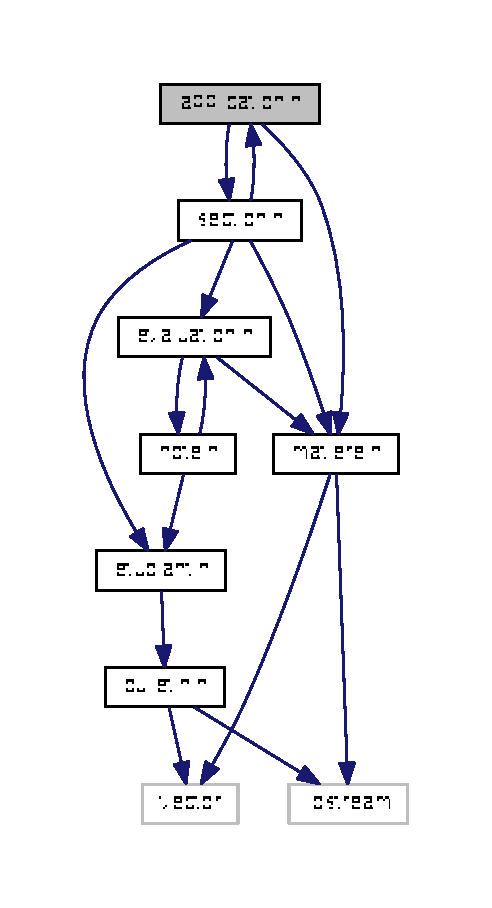
\includegraphics[width=236pt]{application_8h__incl}
\end{center}
\end{figure}
Ce graphe montre quels fichiers incluent directement ou indirectement ce fichier \+:\nopagebreak
\begin{figure}[H]
\begin{center}
\leavevmode
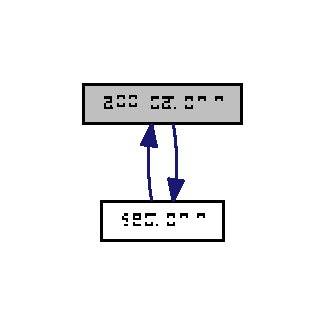
\includegraphics[width=156pt]{application_8h__dep__incl}
\end{center}
\end{figure}
\subsection*{Classes}
\begin{DoxyCompactItemize}
\item 
class \hyperlink{class_application}{Application}
\begin{DoxyCompactList}\small\item\em classe instanciée une fois dans le main \end{DoxyCompactList}\end{DoxyCompactItemize}


\subsection{Description détaillée}
\begin{DoxyAuthor}{Auteur}
B\+A\+Y\+E\+U\+X Rémy 
\end{DoxyAuthor}
\begin{DoxyVersion}{Version}
0.\+1 
\end{DoxyVersion}

\hypertarget{etudiant_8h}{\section{Référence du fichier etudiant.\+h}
\label{etudiant_8h}\index{etudiant.\+h@{etudiant.\+h}}
}
{\ttfamily \#include \char`\"{}bulletin.\+h\char`\"{}}\\*
Graphe des dépendances par inclusion de etudiant.\+h\+:
\nopagebreak
\begin{figure}[H]
\begin{center}
\leavevmode
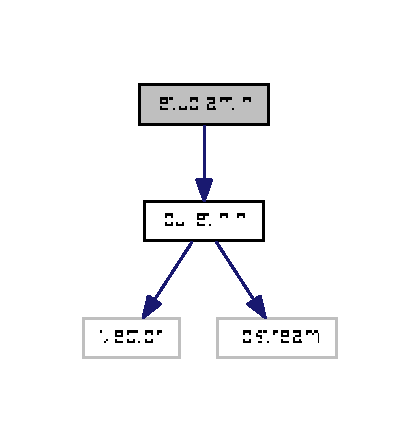
\includegraphics[width=201pt]{etudiant_8h__incl}
\end{center}
\end{figure}
Ce graphe montre quels fichiers incluent directement ou indirectement ce fichier \+:
\nopagebreak
\begin{figure}[H]
\begin{center}
\leavevmode
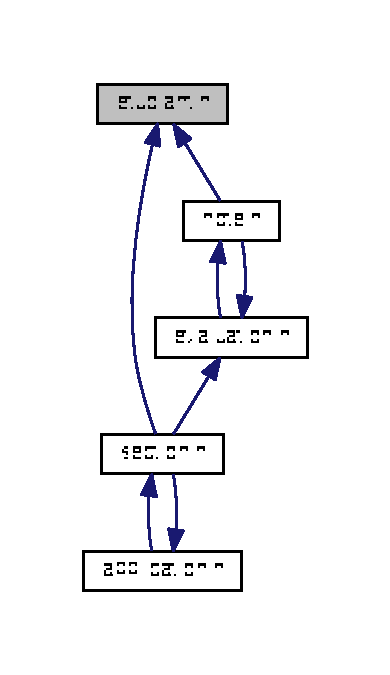
\includegraphics[width=187pt]{etudiant_8h__dep__incl}
\end{center}
\end{figure}
\subsection*{Classes}
\begin{DoxyCompactItemize}
\item 
class \hyperlink{class_etudiant}{Etudiant}
\begin{DoxyCompactList}\small\item\em classe dont il peux exister plusieur instance dans la section \end{DoxyCompactList}\end{DoxyCompactItemize}


\subsection{Description détaillée}
\begin{DoxyAuthor}{Auteur}
B\+A\+Y\+E\+U\+X Rémy 
\end{DoxyAuthor}
\begin{DoxyVersion}{Version}
0.\+1 
\end{DoxyVersion}

\hypertarget{matiere_8h}{\section{Référence du fichier matiere.\+h}
\label{matiere_8h}\index{matiere.\+h@{matiere.\+h}}
}
{\ttfamily \#include $<$vector$>$}\\*
{\ttfamily \#include $<$iostream$>$}\\*
Graphe des dépendances par inclusion de matiere.\+h\+:\nopagebreak
\begin{figure}[H]
\begin{center}
\leavevmode
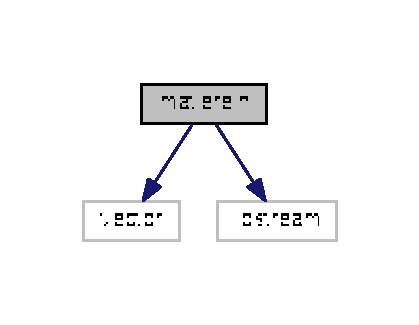
\includegraphics[width=201pt]{matiere_8h__incl}
\end{center}
\end{figure}
Ce graphe montre quels fichiers incluent directement ou indirectement ce fichier \+:\nopagebreak
\begin{figure}[H]
\begin{center}
\leavevmode
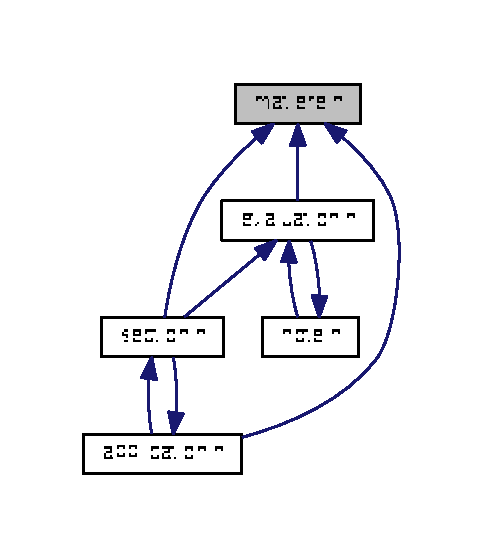
\includegraphics[width=232pt]{matiere_8h__dep__incl}
\end{center}
\end{figure}
\subsection*{Classes}
\begin{DoxyCompactItemize}
\item 
class \hyperlink{class_matiere}{Matiere}
\begin{DoxyCompactList}\small\item\em classe dont il peux exister plusieur instance dans l'application \end{DoxyCompactList}\end{DoxyCompactItemize}


\subsection{Description détaillée}
\begin{DoxyAuthor}{Auteur}
B\+A\+Y\+E\+U\+X Rémy 
\end{DoxyAuthor}
\begin{DoxyVersion}{Version}
0.\+1 
\end{DoxyVersion}

\hypertarget{section_8h}{\section{Référence du fichier section.\+h}
\label{section_8h}\index{section.\+h@{section.\+h}}
}
{\ttfamily \#include \char`\"{}application.\+h\char`\"{}}\\*
{\ttfamily \#include \char`\"{}etudiant.\+h\char`\"{}}\\*
{\ttfamily \#include \char`\"{}evaluation.\+h\char`\"{}}\\*
{\ttfamily \#include \char`\"{}matiere.\+h\char`\"{}}\\*
Graphe des dépendances par inclusion de section.\+h\+:
\nopagebreak
\begin{figure}[H]
\begin{center}
\leavevmode
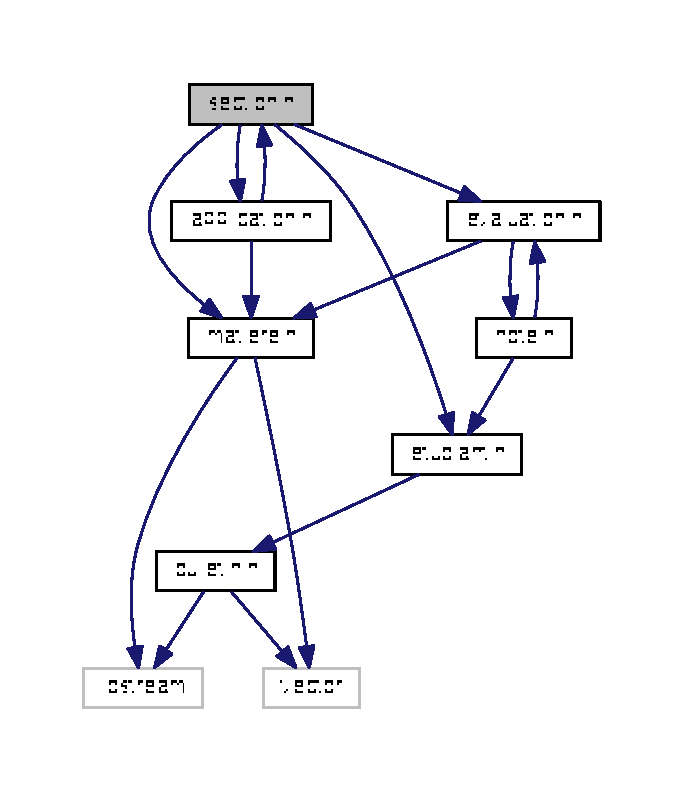
\includegraphics[width=328pt]{section_8h__incl}
\end{center}
\end{figure}
Ce graphe montre quels fichiers incluent directement ou indirectement ce fichier \+:\nopagebreak
\begin{figure}[H]
\begin{center}
\leavevmode
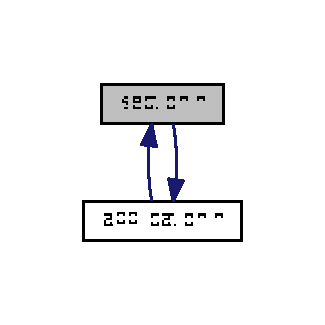
\includegraphics[width=156pt]{section_8h__dep__incl}
\end{center}
\end{figure}
\subsection*{Classes}
\begin{DoxyCompactItemize}
\item 
class \hyperlink{class_section}{Section}
\begin{DoxyCompactList}\small\item\em classe dont il peux exister plusieur instance dans l'application \end{DoxyCompactList}\end{DoxyCompactItemize}


\subsection{Description détaillée}
\begin{DoxyAuthor}{Auteur}
B\+A\+Y\+E\+U\+X Rémy 
\end{DoxyAuthor}
\begin{DoxyVersion}{Version}
0.\+1 
\end{DoxyVersion}

%--- End generated contents ---

% Index
\newpage
\phantomsection
\addcontentsline{toc}{chapter}{Index}
\printindex

\end{document}
